\documentclass[aspectratio=169,xcolor=dvipsnames]{beamer}

%==============================================================================
% PACKAGES & THEME
%==============================================================================
\usepackage[utf8]{inputenc}
\usepackage[T1]{fontenc}
\usepackage{amsmath,amssymb,mathtools}
\usepackage{graphicx}
\usepackage{booktabs}
\usepackage{hyperref}
\usepackage{xcolor}
\usepackage{tikz}
\usepackage{subcaption}
\usepackage[authoryear]{natbib}
\usepackage{multirow}

\usetikzlibrary{shapes.geometric, arrows, positioning, shadows, fit}

% Modern color palette
\definecolor{MainBlue}{HTML}{1A237E}
\definecolor{AccentTeal}{HTML}{009688}
\definecolor{AccentOrange}{HTML}{FF6D00}
\definecolor{SoftGrey}{HTML}{F5F5F5}
\definecolor{DarkGrey}{HTML}{424242}

\usetheme{metropolis} % Clean, modern theme
\metroset{block=fill, sectionpage=progressbar, progressbar=frametitle}

\setbeamercolor{palette primary}{bg=MainBlue, fg=white}
\setbeamercolor{progress bar}{fg=AccentTeal}
\setbeamercolor{frametitle}{bg=MainBlue, fg=white}

% Custom commands
\newcommand{\I}[1]{\mathbf{1}\{#1\}}
\newcommand{\E}{\mathbb{E}}

%==============================================================================
% TITLE DATA
%==============================================================================
\title{Predictive Stability Under Structural Breaks}
\subtitle{Monte Carlo Simulation}
\author{Aadya Khatavkar \and Bakhodir Izzatulloev \and Mahir Baylarov}
\date{Winter Semester 2025/26}
\institute{University of Bonn}

\begin{document}

% 1. Title Page
\begin{frame}[plain]
  \titlepage
\end{frame}

% 2. Motivation: The "Infographic" Slide
\begin{frame}{Motivation: Why Adapt?}
  \begin{columns}
    \begin{column}{0.6\textwidth}
      \begin{itemize}
        \item \textbf{The Reality:} Economic data is rarely stable (Crisis, Policy, Tech).
        \item \textbf{The Failure:} Global models average across regimes $\to$ Massive Bias.
        \item \textbf{The Goal:} Navigate shifts in \textbf{Mean}, \textbf{Variance}, and \textbf{Parameter}.
      \end{itemize}
    \end{column}
    \begin{column}{0.4\textwidth}
      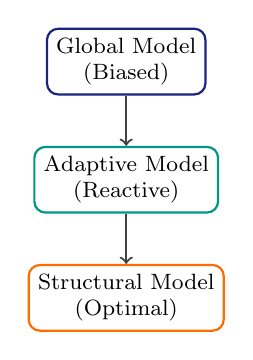
\begin{tikzpicture}[node distance=1.5cm, every node/.style={fill=white, font=\footnotesize}, align=center]
        \node (a) [draw=MainBlue, thick, rounded corners] {Global Model\\(Biased)};
        \node (b) [below of=a, draw=AccentTeal, thick, rounded corners] {Adaptive Model\\(Reactive)};
        \node (c) [below of=b, draw=AccentOrange, thick, rounded corners] {Structural Model\\(Optimal)};
        \draw [->, thick, DarkGrey] (a) -- (b);
        \draw [->, thick, DarkGrey] (b) -- (c);
      \end{tikzpicture}
    \end{column}
  \end{columns}
  \vspace{0.5cm}
  \begin{block}{Research Question}
    How do different forecasting strategies react to structural breaks across various simulation scenarios?
  \end{block}
\end{frame}

% 3. Literature Pillars (Concise table)
\begin{frame}{Literature Review: Key Authors}
  \begin{center}
    \renewcommand{\arraystretch}{1.2}
    \begin{tabular}{lp{10cm}}
      \toprule
      \textbf{Pillar} & \textbf{Foundational Contribution} \\
      \midrule
      \textcolor{MainBlue}{\textbf{Evidence}}   & \textbf{Stock \& Watson (1996)}: Document pervasive instability and the cost of ignoring breaks. \\
      \textcolor{MainBlue}{\textbf{Dynamics}}   & \textbf{Koop \& Potter (2005)}: Argue nonlinearity is often unmodeled structural change. \\
      \textcolor{MainBlue}{\textbf{Trade-offs}} & \textbf{Boot \& Pick (2020)}: Modeling breaks depends on size, timing, and persistence. \\
      \textcolor{MainBlue}{\textbf{Adaptive}}   & \textbf{Siliverstovs \& van Dijk (2002)}: Adaptive methods beat fixed-parameter models. \\
      \textcolor{MainBlue}{\textbf{Regimes}}    & \textbf{Hamilton (1989)}: Markov-Switching for recurring, stochastic regime shifts. \\
      \bottomrule
    \end{tabular}
  \end{center}
\end{frame}

% 4. Data-Generating Process (DGP)
\begin{frame}{Data-Generating Process (DGP)}
  \begin{itemize}
    \item \textbf{Pure Simulation Framework:} No empirical data; all results derived from controlled Monte Carlo experiments.
    \item \textbf{Baseline Structure:} DGP process as the engine for structural change:
    \[ y_t = \mu_t + \phi_t y_{t-1} + \varepsilon_t, \quad \varepsilon_t \sim \text{Dist}(0, \sigma_t^2) \]
    \item \textbf{Sources of Instability (Ceteris Paribus):}
    \begin{itemize}
      \item \textbf{Mean Shifts:} Changes in mean level ($\mu_t$).
      \item \textbf{Variance Shifts:} Changes in $\sigma_t^2$ (Volatility).
      \item \textbf{Parameter Shifts:} Changes in autoregressive parameter $\phi_t$.
    \end{itemize}
    \item \textbf{Persistence Instability Designs:}
    \begin{itemize}
      \item \textbf{Single Break:} Deterministic shifts at a specific time point.
      \item \textbf{Recurring Breaks:} Shifts governed by a \textbf{finite-state Markov process}.
    \end{itemize}
    \item \textbf{Design Philosophy:} Isolate single sources of instability while holding others fixed to evaluate predictive stability.
  \end{itemize}
\end{frame}


% 5. Result 1.1: Single Mean Break Overview
\begin{frame}{Result 1.1: Single Mean Break Overview}
  \begin{columns}[T]
    \begin{column}{0.48\textwidth}
       \centering \scriptsize \textbf{RMSE} \\
       \includegraphics[width=0.8\textwidth]{../../figures/mean/single_break_RMSE.png} \\ \vspace{0.1cm}
       \centering \scriptsize \textbf{Bias Analysis} \\
       \includegraphics[width=0.8\textwidth]{../../figures/mean/single_break_Bias.png}
    \end{column}
    \begin{column}{0.48\textwidth}
       \centering \scriptsize \textbf{MAE} \\
       \includegraphics[width=0.8\textwidth]{../../figures/mean/single_break_MAE.png} \\ \vspace{0.1cm}
       \centering \scriptsize \textbf{Example Series} \\
       \includegraphics[width=0.8\textwidth]{../../figures/mean/single_break_seasonal_series.png}
    \end{column}
  \end{columns}
  \vspace{0.2cm}
  {\scriptsize
  \begin{itemize}
    \item \textbf{Finding:} \textbf{SARIMA Rolling} beats global by 15-20\% RMSE.
    \item \textbf{Oracle:} Known break dates reduce RMSE by an additional 10\%.
    \item \textbf{Seasonality:} SARIMA effectively handles periodic components.
  \end{itemize}
  }
\end{frame}

% 6. Result 1.2: Multiple Mean Break Overview
\begin{frame}{Result 1.2: Multiple Mean Break Overview}
  \begin{columns}[T]
    \begin{column}{0.48\textwidth}
       \centering \scriptsize \textbf{RMSE (Single vs Multiple)} \\
       \includegraphics[width=0.9\textwidth]{../../figures/mean/compare_RMSE_single_vs_multiple.png}
    \end{column}
    \begin{column}{0.48\textwidth}
       \centering \scriptsize \textbf{MAE (Single vs Multiple)} \\
       \includegraphics[width=0.9\textwidth]{../../figures/mean/compare_MAE_single_vs_multiple.png}
    \end{column}
  \end{columns}
  \begin{center}
     \scriptsize \textbf{Example Series with Multiple Breaks} \\
     \includegraphics[width=0.6\textwidth]{../../figures/mean/multiple_break_seasonal_series.png}
  \end{center}
  \vspace{0.1cm}
  {\scriptsize
  \begin{itemize}
    \item \textbf{Complexity:} Multiple breaks degrade performance; SARIMA + Dummies remains consistent.
  \end{itemize}
  }
\end{frame}

% 7. Result 1.3: Single Mean Break Performance (Numerical)
\begin{frame}{Result 1.3: Single Mean Break Performance (Numerical)}
  \small
  \begin{table}
    \centering
    \begin{tabular}{lccccc}
      \toprule
      \textbf{Method} & \textbf{RMSE} & \textbf{MAE} & \textbf{Bias} & \textbf{N} & \textbf{Fails} \\
      \midrule
      SARIMA + Break Dummy (Oracle) & 1.455 & 1.194 & 1.006 & 200 & 0 \\
      Simple Exp. Smoothing (SES) & 1.496 & 1.225 & 1.015 & 200 & 0 \\
      SARIMA Rolling & 1.525 & 1.257 & 1.029 & 200 & 0 \\
      SARIMA + Estimated Break & 1.635 & 1.368 & 1.243 & 200 & 0 \\
      SARIMA Global & 1.692 & 1.423 & 1.302 & 200 & 0 \\
      \bottomrule
    \end{tabular}
    \caption{Mean metrics across 200 replications ($T=300$)}
  \end{table}
  \begin{itemize}
    \item \textbf{Best Performer:} Oracle dummy model (benchmarking the theoretical limit).
    \item \textbf{Observation:} Even simple SES outperforms global SARIMA by discarding history.
  \end{itemize}
\end{frame}

% 8. Result 1.4: Mean Break Comparison (Numerical)
\begin{frame}{Result 1.4: Mean Break Comparison (Numerical)}
  \centering
  \resizebox{0.75\textwidth}{!}{
    \begin{tabular}{lcccccc}
      \toprule
      \textbf{Method} & \textbf{RMSE} & \textbf{MAE} & \textbf{Bias} & \textbf{N} & \textbf{Fails} & \textbf{Scenario} \\
      \midrule
      SARIMA + 2 Dummies (Oracle) & 0.985 & 0.781 & 0.106 & 200 & 0 & Multiple \\
      SARIMA Global & 1.042 & 0.836 & -0.045 & 200 & 0 & Multiple \\
      SARIMA + 2 Breaks (Grid) & 1.046 & 0.845 & -0.125 & 200 & 0 & Multiple \\
      Holt--Winters Seasonal & 1.094 & 0.857 & -0.001 & 200 & 0 & Multiple \\
      SARIMA Rolling & 1.122 & 0.884 & 0.299 & 200 & 0 & Multiple \\
      \midrule
      SARIMA + Dummy (Oracle) & 1.455 & 1.194 & 1.006 & 200 & 0 & Single \\
      SES (level smoothing) & 1.496 & 1.225 & 1.015 & 200 & 0 & Single \\
      SARIMA Rolling & 1.525 & 1.257 & 1.029 & 200 & 0 & Single \\
      SARIMA + Break (Grid) & 1.635 & 1.368 & 1.243 & 200 & 0 & Single \\
      SARIMA Global & 1.692 & 1.423 & 1.302 & 200 & 0 & Single \\
      \bottomrule
    \end{tabular}
  }
  \vspace{0.1cm}
  {\small
  \begin{itemize}
    \item \textbf{Multiple Breaks:} Paradoxically lower RMSE for Global models due to variance.
    \item \textbf{Single Break:} Clear dominance of adaptive (Rolling/Oracle) methods.
  \end{itemize}
  }
\end{frame}

% 9. Result 2.1: Parameter Breaks - Single Shift
\begin{frame}{Result 2.1: Parameter Breaks - Single Shift}
  \begin{columns}[T]
    \column{0.33\textwidth}
    \centering \small \textbf{DGP Visualization} \\
    \includegraphics[width=\textwidth]{Single break DGP.png}
    \column{0.33\textwidth}
    \centering \small \textbf{Error Distributions} \\
    \includegraphics[width=\textwidth]{Distribution Single break.png}
    \column{0.33\textwidth}
    \centering \small \textbf{RMSE over Dof} \\
    \includegraphics[width=\textwidth]{RMSE over Dof single break.png}
  \end{columns}
  \vspace{0.2cm}
  \begin{itemize}
    \item \textbf{Scenario:} Shift in persistence $\phi_1 \to \phi_2$.
    \item \textbf{Impact:} Leads to systematic under/over-estimation of memory.
  \end{itemize}
\end{frame}

% 10. Result 2.2: Recurring Parameter Breaks
\begin{frame}{Result 2.2: Recurring Parameter Breaks (RMSE/MAE/Bias)}
  \begin{columns}[T]
    \column{0.33\textwidth}
    \centering \small \textbf{RMSE} \\
    \includegraphics[width=\textwidth]{RMSE recurring.png}
    \column{0.33\textwidth}
    \centering \small \textbf{MAE} \\
    \includegraphics[width=\textwidth]{MAE recurring.png}
    \column{0.33\textwidth}
    \centering \small \textbf{Bias} \\
    \includegraphics[width=\textwidth]{Bias recurring.png}
  \end{columns}
  \vspace{0.2cm}
  \begin{itemize}
    \item \textbf{Markov Switching:} Best at capturing recurring shifts.
  \end{itemize}
\end{frame}

% 11. Result 2.3: Persistence Analysis
\begin{frame}{Result 2.3: Persistence Analysis \& Recurring DGP}
  \begin{columns}
    \begin{column}{0.5\textwidth}
       \centering \textbf{DGP Recurring Break} \\
       \includegraphics[width=0.9\textwidth]{GDP_recurring break.png}
    \end{column}
    \begin{column}{0.5\textwidth}
       \centering \textbf{Recurring Distribution} \\
       \includegraphics[width=0.9\textwidth]{Distribution recurring.png}
    \end{column}
  \end{columns}
  \vspace{0.2cm}
  {\small
  \begin{itemize}
    \item As persistence increases, regime durations lengthen and the series exhibits extended periods of distinct dynamics. In the high-persistence case, regime switches are rare and regime spells become long but remain stochastic, illustrating near-permanent yet non-degenerate parameter regimes.
  \end{itemize}
  }
\end{frame}

% 12. Result 3.1: Volatility Shifts
\begin{frame}{Result 3.1: Volatility Shifts (Variance Breaks)}
  \begin{columns}
    \begin{column}{0.5\textwidth}
      \begin{itemize}
        \item \textbf{Winner:} \textbf{GARCH(1,1)} adapts fastest to variance shifts.
        \item \textbf{Insight:} Rolling windows must be small ($w < 50$) to capture sudden volatility jumps.
        \item \textbf{Loss Surface:} Clear U-shape showing window size trade-off.
      \end{itemize}
    \end{column}
    \begin{column}{0.5\textwidth}
       \includegraphics[width=\textwidth]{../../figures/variance/variance_forecasts_comparison.png}
    \end{column}
  \end{columns}
\end{frame}

% 13. Result 3.2: Variance Robustness
\begin{frame}{Result 3.2: Variance Robustness: Loss Surfaces}
  \begin{itemize}
    \item \textbf{Parameter Sensitivity:} Heatmap showing RMSE across varying window sizes and break magnitudes.
    \item \textbf{Optimal Region:} Clear visualization of the stable regions for rolling window adaptation.
    \item \textbf{Insight:} Demonstrates the bias-variance tradeoff as the "U-shape" loss across scenarios.
  \end{itemize}
  \begin{center}
     \includegraphics[width=0.85\textwidth]{../../figures/variance/variance_loss_surfaces.png}
  \end{center}
\end{frame}

% 14. Result 3.3: Variance Performance (Numerical)
\begin{frame}{Result 3.3: Variance Performance (Numerical)}
  \small
  \begin{table}
    \centering
    \begin{tabular}{lcccc}
      \toprule
      \textbf{Scenario} & \textbf{ARIMA Global} & \textbf{ARIMA Rolling} & \textbf{GARCH(1,1)} & \textbf{Post-Break} \\
      \midrule
      Variance 1.5x & 1.807 & 1.831 & 1.805 & 1.848 \\
      Variance 2.0x & 2.417 & 2.448 & 2.414 & 2.472 \\
      Variance 3.0x & 3.620 & 3.677 & 3.613 & 3.688 \\
      Variance 5.0x & 6.231 & 6.306 & 6.219 & 6.341 \\
      \bottomrule
    \end{tabular}
    \caption{RMSE across 200 Monte Carlo replications ($T=400$)}
  \end{table}
  \vspace{0.2cm}
  \begin{itemize}
    \item \textbf{Observation:} GARCH consistently achieves the lowest RMSE across all magnitudes.
    \item \textbf{Adaptation:} Global ARIMA suffers from persistent bias after the shock.
    \item \textbf{Windowing:} Rolling window performance is sensitive to the $0.6\sqrt{T}$ rule.
  \end{itemize}
\end{frame}

% 15. Future Research
\begin{frame}{Future Research Directions}
  \begin{itemize}
    \item \textbf{Complex Breaks:} Simultaneous shifts in mean, variance, and parameters.
    \item \textbf{Empirical Tests:} Validating simulation results on GDP and stock returns.
    \item \textbf{Probabilistic Forecasting:} Density scores and improved uncertainty quantification.
    \item \textbf{Multivariate Systems:} Extending breaks to high-dimensional VAR systems.
    \item \textbf{Hybrid Modeling:} Integrating machine learning with classical structural models.
  \end{itemize}
  \vfill
  \centering \footnotesize \textit{Moving from controlled simulations to real-world complexity.}
\end{frame}

% 16. References
\begin{frame}{Selected References}
  \tiny
  \nocite{stock1996, koop2005, boot2020, siliverstovs2002, hamilton1989, cai2007, delgado2000, koo2012, perron2006, pesaran2013_jo, kooseo2015}
  \bibliographystyle{apalike}
  \bibliography{bibliography}
\end{frame}

% 17. Thank You
\begin{frame}[plain]
  \begin{center}
    \vspace{2cm}
    \Huge \textcolor{MainBlue}{\textbf{Thank You!}} \\
    \vspace{1cm}
    \large \textbf{Questions?} \\
    \vspace{1.5cm}
    \footnotesize \texttt{github.com/qonlab/structural-break-forecasting}
  \end{center}
\end{frame}

\end{document}
